% Isolated author-review copy. The formal manuscript is not modified.
\documentclass[conference]{IEEEtran}

\usepackage{amsmath,amssymb}
\usepackage{booktabs}
\usepackage{graphicx}
\usepackage{tabularx}
\usepackage{stfloats}
\usepackage{capt-of}
\usepackage{url}
\usepackage{balance}
\setcounter{dbltopnumber}{2}
\renewcommand{\dbltopfraction}{0.95}
\renewcommand{\textfraction}{0.05}
\setlength{\emergencystretch}{1em}

\title{Measurement-Based Multipath Characterization of GPS L1 C/A Signals for Vehicular Satellite-to-Ground Links in Challenging Environments}

\author{\IEEEauthorblockN{Liang Feng}
\IEEEauthorblockA{Tongji University, Shanghai, China\\2432132@tongji.edu.cn}}

\begin{document}
\maketitle

\begin{abstract}
Reliable satellite-based positioning for connected and automated vehicles is challenged by reflection-rich propagation and rapidly changing satellite-to-ground geometry in dense urban and mountain/valley roads. As terrestrial and non-terrestrial systems become increasingly integrated for 6G localization, measurement-based characterization of mobile satellite-to-ground propagation remains relevant to positioning evaluation. This paper presents a measurement-based framework for extracting and statistically characterizing GPS L1 C/A multipath components (MPCs) from moving-vehicle measurements in two challenging environments. Navigation-data alignment is used to form coherent 40-ms observations for each tracked satellite. The space-alternating generalized expectation-maximization (SAGE) algorithm estimates the delay, Doppler, and complex gain of candidate MPCs, and a temporal-consistency criterion retains persistent MPC observations. The analysis uses 518 persistent MPC observations from 236 satellite tracks. Excess delay is represented by environment-specific lognormal models, signed relative Doppler by a track-balanced empirical cumulative distribution, and relative power by a two-component Gaussian mixture model selected after scene-held-out mixture-complexity checks. A connected two-line model describes the mean power--delay trend. The resulting path-level descriptions provide measurement-based inputs for simplified vehicular satellite-to-ground simulation and are relevant to the evaluation of GNSS and NTN-assisted localization in challenging propagation conditions.
\end{abstract}

\begin{IEEEkeywords}
GNSS multipath, vehicular satellite-to-ground propagation, GPS L1 C/A, SAGE, NTN-assisted localization, channel modeling.
\end{IEEEkeywords}

\section{Introduction}
Integrated terrestrial and non-terrestrial networks (NTNs) are becoming an important part of the evolution from 5G-Advanced toward 6G, with satellite systems considered not only for ubiquitous connectivity but also for positioning and sensing \cite{ntnRel1718_2024,ntn6gSurvey2024,ntnLocalization2023,tnNtnLocalization2025}. For connected and automated vehicles, this evolution is relevant because positioning must remain available under mobility and heterogeneous coverage, while future V2X architectures increasingly combine terrestrial and non-terrestrial resources \cite{v2x6g2025,leoMobilityPositioning2026}.

GNSS remains the primary satellite-based positioning technology for road vehicles, but dense urban streets and mountain/valley roads create challenging satellite-to-ground propagation conditions. Reflections from buildings and terrain produce delayed and Doppler-shifted replicas whose relative strength changes as the vehicle moves. These propagation effects can complicate signal tracking and positioning in dynamic road environments. Earlier GPS multipath studies characterized receiver-level effects through carrier-to-noise-density ratio, pseudorange error, carrier-phase error, and multipath indicators \cite{eissfeller1996gpsdynamic,mora1998multipath,bilich2007snr,xie2011vehicular,beitler2015cmcd}. Such quantities describe receiver-level consequences of multipath, but they do not directly provide the delay, Doppler, and complex gain of individual multipath components.

Traditional land-mobile satellite channel models organize reflections in a time-varying channel impulse response or power-delay profile \cite{lehner2005lms}. At the path-parameter level, the space-alternating generalized expectation-maximization algorithm can estimate individual MPC parameters from complex baseband measurements by updating subsets of channel parameters in sequence \cite{fessler1994sage,fleury1999sage}. Gaussian mixtures provide one way to describe multimodal measured parameter distributions \cite{selim2016mog}. A complementary measurement perspective is therefore to resolve individual MPCs from real moving-vehicle observations and characterize their delay, signed relative Doppler, and relative power across distinct challenging propagation environments. Such path-resolved measurements can complement system-level studies of vehicular satellite positioning and integrated TN/NTN localization by providing empirical propagation inputs for controlled simulation and receiver evaluation.

This work combines per-satellite MPC extraction with environment-specific statistical characterization using real GPS L1 C/A measurements collected from a moving vehicle. Navigation-data alignment forms coherent observations for each tracked satellite, SAGE estimates MPC delay, Doppler, and complex gain, and temporal-consistency screening retains persistent MPC observations. The statistical analysis compares Urban and Mountain/Valley environments and evaluates model complexity using complete-scene held-out validation before selecting the paper-facing parameter descriptions. Although the measurements use GPS L1 C/A rather than an NR-NTN air interface, the resulting path-level evidence is relevant to challenging vehicular satellite-to-ground propagation and NTN-assisted localization evaluation. Sections II--IV present the measurements and per-satellite processing, MPC estimation and statistical descriptions, and experimental results, respectively.

\section{Measurements and Signal Processing}
\subsection{Measurement Setup}
The measurement system uses a TEST-TREE RF-Catcher V2 and a roof-mounted GNSS dome antenna. The antenna is right-hand circularly polarized and has a 40-dB active gain. The receiver records GPS L1 C/A at 1575.42 MHz \cite{gpsis200n2022}. The sampling rate is 10.23 MHz. Samples are stored as interleaved, little-endian, signed 16-bit I/Q values.

The measurements were collected while the vehicle traveled along two types of roads. Urban routes are surrounded by dense buildings, whereas Mountain/Valley routes pass through mountainous or valley terrain. These route classes are treated as two challenging vehicular satellite-to-ground propagation settings with distinct surrounding structures; the analysis compares their path-level statistics without ranking one environment as universally more severe.

\subsection{Per-Satellite Multipath Processing}
GNSS-SDR first tracks each visible satellite and decodes its navigation data \cite{fernandez2011gnsssdr}. Because different satellites use different pseudorandom-noise codes, each tracked satellite is processed in a separate signal stream. Fig.~\ref{fig:workflow} summarizes this processing flow. Each GPS L1 C/A navigation bit lasts 20 ms; thus, a 40-ms observation may contain a bit transition that reverses the signal sign. The decoded bit signs are removed before coherent observations are formed. Correlation screening identifies observations that may contain an additional signal component. SAGE then estimates MPC parameters for each selected observation. A temporal-consistency check compares adjacent observations and retains persistent MPC observations for the statistical analysis.

\begin{figure*}[t]
\centering
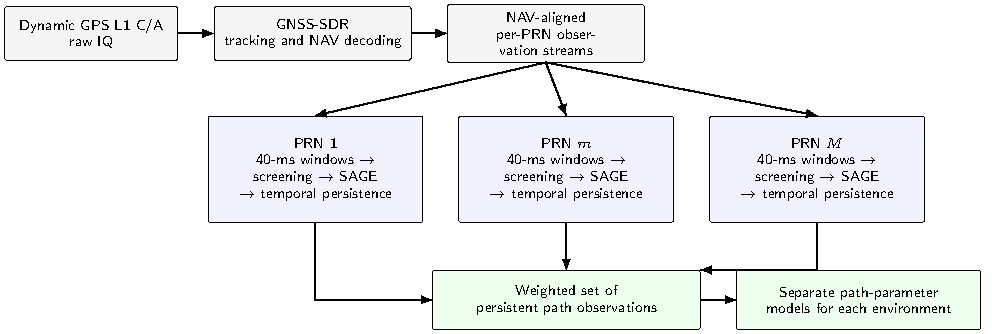
\includegraphics[width=0.96\textwidth]{figures/figure1_multisatellite.pdf}
\caption{Measurement and per-satellite MPC processing flow.}
\label{fig:workflow}
\end{figure*}

\section{Multipath Component Estimation and Statistical Modeling}
\subsection{SAGE-Based MPC Estimation}
Let $m$ denote one tracked satellite-to-receiver channel. Its complex baseband signal is
\begin{equation}
r_m(t)=\sum_{\ell=0}^{L_m-1}\alpha_{m,\ell}s_m(t-\tau_{m,\ell})
e^{j2\pi\nu_{m,\ell}t}+n_m(t),
\label{eq:signal}
\end{equation}
where $s_m(t)$ is the aligned C/A-code waveform and $n_m(t)$ is noise. MPC $\ell$ has complex gain $\alpha_{m,\ell}$, delay $\tau_{m,\ell}$, and Doppler frequency shift $\nu_{m,\ell}$. The earliest estimated component ($\ell=0$) is used only as a relative reference and is not interpreted as a verified line-of-sight component.

The SAGE algorithm updates one MPC at a time \cite{fessler1994sage,fleury1999sage}. Operationally, the current reconstructions of the other MPCs are subtracted before the target MPC is re-estimated. For target MPC $\ell$, the E-step forms a conditional hidden-data estimate by subtracting the current contributions of the other MPCs from the received observation:
\begin{equation}
\mathbf r_{m,\ell}=\mathbf r_m-\sum_{k\ne\ell}\hat\alpha_{m,k}
\mathbf q_m(\hat\tau_{m,k},\hat\nu_{m,k}).
\label{eq:hidden}
\end{equation}
The M-step updates the delay and Doppler frequency shift of the target MPC by
\begin{equation}
(\hat\tau_{m,\ell},\hat\nu_{m,\ell})=
\operatorname*{arg\,max}_{\tau,\nu}
\frac{|\mathbf q_m(\tau,\nu)^H\mathbf r_{m,\ell}|^2}
{\mathbf q_m(\tau,\nu)^H\mathbf q_m(\tau,\nu)},
\label{eq:sage}
\end{equation}
where $\mathbf q_m(\tau,\nu)$ is a sampled code replica with fractional delay and Doppler. After all MPCs have been updated in one sweep, their complex gains are jointly estimated by least squares.

Equation~\eqref{eq:sage} selects the delay--Doppler pair with the highest normalized correlation to the conditional hidden-data estimate. A coarse correlation search provides the initial parameter values. The delay is then refined with fractional-sample code replicas spaced by 0.1 sample within a $\pm0.8$-sample neighborhood. The Doppler frequency shift is searched within $\pm30$ Hz of the tracking estimate in 5-Hz steps. The iterations terminate after 10 sweeps or when the relative change in the residual sum of squares (RSS) falls below $10^{-6}$.

For each 40-ms observation, four candidate models are evaluated, with one, two, three, or four MPCs. The path count is selected by comparing the Bayesian information criterion and residual sum of squares (RSS) across these candidates. This comparison balances signal representation against model complexity.

\subsection{Persistent MPC Observations}
After local estimation, MPC estimates from adjacent observations are compared. A match is declared only when the excess-delay, signed relative Doppler, and relative-power differences are simultaneously no greater than 1.5 samples, 40 Hz, and 10 dB, respectively. An MPC is labeled persistent when matching estimates occur in at least three consecutive observations. A 40-ms observation is used for modeling only when every nonreference MPC satisfies this condition. The parameters at the center time are then retained as the persistent MPC observation.

For each persistent MPC observation, the three parameters are expressed relative to the reference component:
\begin{equation}
\Delta\tau=\tau_{\ell}-\tau_{0},\quad
\nu_{\rm rel}=\nu_{\ell}-\nu_{0},\quad
P_{\rm rel}=10\log_{10}\frac{|\alpha_{\ell}|^2}{|\alpha_{0}|^2}.
\label{eq:parameters}
\end{equation}
Here, $\Delta\tau$ is the delay relative to the reference component, $\nu_{\rm rel}$ is signed relative Doppler, and $P_{\rm rel}$ is the power relative to the reference component in decibels.

\subsection{Candidate Models and Environment-Specific Statistical Descriptions}
Satellite tracks contain different numbers of persistent MPC observations. Each track is therefore assigned the same total weight, preventing a longer track from dominating the environment-level statistics simply because it contains more observations. If track $j$ contains $n_j$ observations, each observation in that track receives weight $w_i=1/n_j$.

Several parametric distributions were considered for excess delay and relative power in each environment. Candidate distributions were compared using leave-one-scene-out (LOSO) validation: one complete measurement scene was held out, the candidates were fitted to the remaining scenes, and their performance was evaluated on the held-out scene. This was repeated until every scene had been held out once. Model selection used both the predictive likelihood and the maximum weighted CDF deviation,
\begin{equation}
D_w=\max_i\left|\widehat F_w(x_i)-F_\theta(x_i)\right|,
\label{eq:cdf-distance}
\end{equation}
where $\widehat F_w$ is the weighted empirical CDF and $F_\theta$ is the model CDF. Here, $D_w$ is used as a descriptive goodness-of-fit measure: a smaller value indicates closer agreement between the measured and modeled cumulative distributions.

To make model complexity explicit, one-, two-, and three-component one-dimensional Gaussian mixture models were also evaluated for signed relative Doppler and relative power in each environment using the same track weighting and complete-scene leave-one-scene-out protocol. Under the one-standard-error rule applied to scene-held-out negative log predictive density, the diagnostic mixture complexities were $K=2$ for Urban signed relative Doppler, $K=3$ for Mountain/Valley signed relative Doppler, and $K=2$ for relative power in both environments. The Doppler mixtures are used only as complexity diagnostics; the paper retains the track-balanced empirical CDF as its reported Doppler representation so that no parametric mixture law is imposed on the measured signed Doppler distribution. For relative power, the two-component GMM is retained as the paper-facing model.

\begin{table}[t]
\centering
\caption{Diagnostic GMM complexity from complete-scene LOSO validation.}
\label{tab:gmm-complexity}
\scriptsize
\setlength{\tabcolsep}{3pt}
\begin{tabular}{lccc}
\toprule
Quantity & Urban & Mountain/Valley & Reported description\\
\midrule
Signed relative Doppler & $K=2$ & $K=3$ & Empirical CDF\\
Relative power & $K=2$ & $K=2$ & Two-component GMM\\
\bottomrule
\end{tabular}
\end{table}

Signed relative Doppler is represented directly by its track-balanced empirical CDF. For environment $e$, the CDF and its weighted quantiles are defined as
\begin{equation}
\begin{aligned}
\widehat F_{\nu,e}(x)
&=\frac{\sum_{i\in e}w_i\mathbf{1}(\nu_i\le x)}
{\sum_{i\in e}w_i},\\
P_q(e)&=\inf\{x:\widehat F_{\nu,e}(x)\ge q\}.
\end{aligned}
\label{eq:doppler-ecdf}
\end{equation}
Here, $\nu_i$ is the signed relative Doppler of observation $i$. The empirical representation retains the measured signed relative Doppler values and is summarized by $P_{10}$, $P_{50}$, and $P_{90}$.

To represent the observed positive and right-skewed excess-delay distribution, a lognormal form is used:
\begin{equation}
\ln(\Delta\tau-\tau_s)\sim\mathcal N(\mu_\tau,\sigma_\tau^2),
\label{eq:lognormal}
\end{equation}
where $\tau_s$ is a shift, $\exp(\mu_\tau)$ is the scale, and $\sigma_\tau$ controls the spread in the logarithmic domain. The Urban model uses an estimated shift, while the Mountain/Valley model uses $\tau_s=0$.

A two-component Gaussian mixture model (GMM) is used to represent the bimodal structure of the measured relative-power distribution:
\begin{equation}
p(x)=\pi\mathcal N(x;\mu_1,\sigma_1^2)
+(1-\pi)\mathcal N(x;\mu_2,\sigma_2^2).
\label{eq:gmm2}
\end{equation}
The mixing weight $\pi$ gives the relative contribution of the first Gaussian component.

Relative power is also modeled as a function of excess delay. Two line segments with different slopes meet at a common breakpoint $\tau_b$:
\begin{equation}
P(\tau)=
\begin{cases}
P_b+b_1(\tau-\tau_b), & \tau<\tau_b,\\
P_b+b_2(\tau-\tau_b), & \tau\ge\tau_b.
\end{cases}
\label{eq:piecewise}
\end{equation}
This connected model allows the mean rate of power decrease to differ between low-delay and high-delay MPCs while keeping the mean trend continuous. The fitted delay and power distributions and the track-balanced empirical CDF of signed relative Doppler provide complementary parameter descriptions for each environment.

Together, these representations characterize the retained MPC parameters at the path level for each environment. The selected forms are also consistent with the main structures observed in the measured data.

\section{Statistical Modeling Results}
\begin{figure*}[!t]
\centering
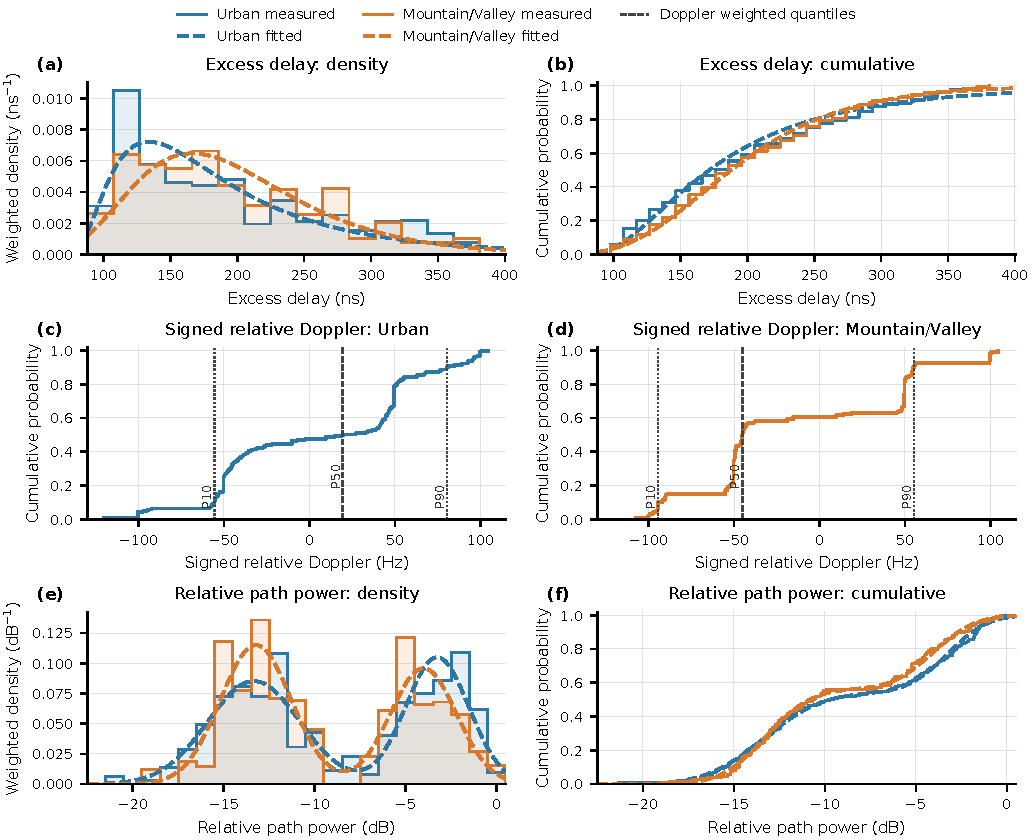
\includegraphics[width=0.98\textwidth]{../../figures/figure2_parameter_distributions.pdf}
\caption{Measured path-parameter distributions and statistical descriptions: (a)--(b) excess delay, (c)--(d) track-balanced empirical CDFs of signed relative Doppler for Urban and Mountain/Valley, respectively, and (e)--(f) relative path power. Fitted curves are shown for excess delay and relative power.}
\label{fig:path-distributions}
\end{figure*}

\subsection{Modeling Data and Excess Delay}
The analysis uses 518 persistent MPC observations from 236 satellite tracks, 36 recordings, and 9 measurement scenes. Of these observations, 346 were collected in the Urban environment and 172 in the Mountain/Valley environment.

Fig.~\ref{fig:path-distributions}(a) and (b) show that both excess-delay distributions are right-skewed. The Urban fit has a shift of 68.7 ns, a scale of 102.8 ns, and a log-domain standard deviation of 0.675. The Mountain/Valley fit has a scale of 187.8 ns and a log-domain standard deviation of 0.348. The larger log-domain standard deviation in Urban is consistent with its broader right tail. Table~\ref{tab:model-parameters} lists the model summaries and fit measures.

\subsection{Signed Relative Doppler}
Fig.~\ref{fig:path-distributions}(c) and (d) show the track-balanced empirical CDFs of signed relative Doppler. For Urban, the weighted $P_{10}$, $P_{50}$, and $P_{90}$ values are $-55.6$, $19.5$, and $80.6$ Hz, respectively. The corresponding values for Mountain/Valley are $-94.4$, $-45.1$, and $55.3$ Hz. The Mountain/Valley distribution is shifted toward more negative signed relative Doppler values, as indicated by its more negative $P_{10}$ and median, whereas the Urban median remains positive. The empirical CDF represents the observed distribution without imposing a parametric family.

The complete-scene complexity check selected two Gaussian components for Urban signed relative Doppler and three for Mountain/Valley, as summarized in Table~\ref{tab:gmm-complexity}. These mixture counts are treated only as diagnostics of distributional complexity. The empirical CDF remains the paper-facing Doppler representation because it preserves the measured signed distribution without requiring a parametric mixture interpretation.

\subsection{Relative Power}
Fig.~\ref{fig:path-distributions}(e) and (f) show two relative-power modes in both environments. These values are relative to the earliest component and are not absolute received powers. The means are near $-13$ dB for the weaker mode and $-3$ to $-4$ dB for the stronger mode. Compared with a single-Gaussian fit, the two-component GMM reduces $D_w$ from 0.133 to 0.045 in Urban and from 0.137 to 0.037 in Mountain/Valley. The same complexity check selected two Gaussian components for relative power in both environments, consistent with the two-component paper-facing GMM.

\begin{table*}[!b]
\centering
\caption{Parameters of the environment-specific descriptions.}
\label{tab:model-parameters}
\scriptsize
\setlength{\tabcolsep}{3pt}
\begin{tabularx}{0.98\textwidth}{llXl}
\toprule
Quantity & Environment & Model summary & Fit measure\\
\midrule
Excess delay & Urban & Shifted lognormal: shift $68.7$ ns, scale $102.8$ ns, log-std. $0.675$ & $D_w=0.082$\\
& Mountain/Valley & Lognormal: scale $187.8$ ns, log-std. $0.348$ & $D_w=0.055$\\
Signed relative Doppler & Urban & Track-balanced empirical CDF: $P_{10}=-55.6$, $P_{50}=19.5$, $P_{90}=80.6$ Hz & ---\\
& Mountain/Valley & Track-balanced empirical CDF: $P_{10}=-94.4$, $P_{50}=-45.1$, $P_{90}=55.3$ Hz & ---\\
Relative power & Urban & GMM: $(-13.35,2.53,0.541)$ and $(-3.27,1.74,0.459)$ dB & $D_w=0.045$\\
& Mountain/Valley & GMM: $(-13.24,1.95,0.562)$ and $(-4.03,1.82,0.438)$ dB & $D_w=0.037$\\
Power--delay & Urban & Breakpoint $190.6$ ns; slopes $-3.53$ and $-5.57$ dB/100 ns & RMSE $4.01$ dB\\
& Mountain/Valley & Breakpoint $190.6$ ns; slopes $-6.31$ and $-4.46$ dB/100 ns & RMSE $3.44$ dB\\
\bottomrule
\end{tabularx}
\vspace{-1mm}
\parbox{0.98\textwidth}{\scriptsize For each GMM component, the three numbers are mean, standard deviation, and weight. $D_w$ is the maximum weighted CDF deviation defined in \eqref{eq:cdf-distance} and applies to the fitted delay and relative-power marginals. Signed relative Doppler is summarized by weighted empirical quantiles.}
\end{table*}

\twocolumn[{
\begin{minipage}{\textwidth}
\centering
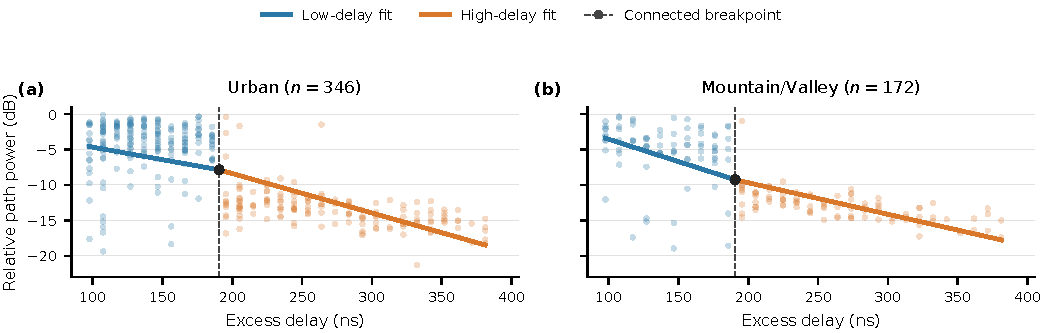
\includegraphics[width=0.94\textwidth]{../../figures/figure3_power_delay.pdf}
\captionof{figure}{Measured relative power and connected two-slope fits versus excess delay.}
\label{fig:power-delay}
\vspace{-2pt}
\end{minipage}
}]

\subsection{Power--Delay Relation}
Fig.~\ref{fig:power-delay} shows the decrease in relative power with increasing excess delay. The connected model has a common breakpoint of 190.6 ns, with separate fitted mean power-decay slopes below and above the breakpoint. In Urban, the slopes are $-3.53$ and $-5.57$ dB per 100 ns before and after the breakpoint; in Mountain/Valley, they are $-6.31$ and $-4.46$ dB per 100 ns. The fitted mean trend is steeper after the breakpoint in Urban and less steep after it in Mountain/Valley. The root-mean-square errors are 4.01 and 3.44 dB, respectively.

For simplified GNSS channel simulation, excess delay and relative power can be sampled from their fitted marginals, signed relative Doppler can be resampled from its track-balanced empirical CDF, and the connected power--delay model can supply the mean delay-dependent power. Together, these descriptions provide MPC parameters for each simulated satellite channel; they do not specify occurrence rates, temporal evolution, or a complete joint stochastic channel model.

\subsection{Relevance to Vehicular Satellite and NTN-Assisted Localization}
These measurements use GPS L1 C/A and therefore do not constitute an NR-NTN air-interface measurement or a 3GPP-compliant NTN channel model. Their relevance to NTN is at the satellite-to-ground propagation and positioning level: the extracted delay, signed relative Doppler, and relative-power statistics describe a moving ground vehicle under challenging real-world propagation conditions. Such measurements can complement system-level studies of vehicular satellite positioning and integrated terrestrial/non-terrestrial localization by providing path-level conditions for simplified simulation and receiver evaluation \cite{tnNtnLocalization2025,v2x6g2025,leoMobilityPositioning2026}.

\section{Conclusion}
This paper presents measurement-based path-level characterization of GPS L1 C/A multipath from moving-vehicle measurements in challenging Urban and Mountain/Valley satellite-to-ground environments. Navigation-data alignment, per-satellite SAGE estimation, and temporal-consistency screening provide persistent MPC observations characterized by excess delay, signed relative Doppler, and relative power. Complete-scene model-complexity checks show that the measured Doppler and relative-power distributions contain structure beyond a single Gaussian representation, while conservative paper-facing descriptions retain an empirical CDF for signed relative Doppler and a two-component GMM for relative power. The resulting models also capture the environment-specific right-skewed excess-delay distributions and the change in mean relative-power decay with excess delay. These path-level descriptions provide measurement-based inputs for simplified satellite-to-ground propagation simulation and receiver evaluation. Although the measurements are based on GPS L1 C/A rather than an NR-NTN air interface, the results provide empirical propagation evidence relevant to vehicular satellite positioning and NTN-assisted localization under challenging propagation conditions.

% \balance
\bibliographystyle{IEEEtran}
\bibliography{references}

\end{document}
